% !TeX root = prob.tex

\section{Ehrenfest model}\label{s.ehrenfest}

\textbf{Problem} The Ehrenfest model is designed to model diffusion of between two containers. In the following diagram there are four particles in the left container and six particles in the right container for a total of $n=10$ particles:
\begin{center}
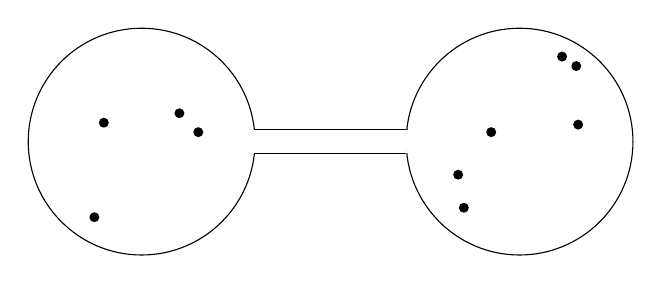
\begin{tikzpicture}[scale=1.2]
\draw (0,0) node {} circle[radius=1.2];
\draw[white,thick] (-6:1.2) arc(-6:6:1.2);
\draw (-6:1.2) -- +(1.63,0);
\draw (6:1.2) -- +(1.63,0);
\fill (-.4,.2) circle[radius=1.5pt];
\fill (.4,.3) circle[radius=1.5pt];
\fill (-.5,-.8) circle[radius=1.5pt];
\fill (.6,.1) circle[radius=1.5pt];
\begin{scope}[xshift=4cm]
\draw (0,0) node {} circle[radius=1.2];
\draw[white,thick] (174:1.2) arc(174:186:1.2);
\fill (-.3,.1) circle[radius=1.5pt];
\fill (.45,.9) circle[radius=1.5pt];
\fill (-.65,-.35) circle[radius=1.5pt];
\fill (.62,.18) circle[radius=1.5pt];
\fill (-.59,-.7) circle[radius=1.5pt];
\fill (.6,.8) circle[radius=1.5pt];
\end{scope}
\end{tikzpicture}
\end{center}
Repeated choose a particle at random with uniform distribution and move it to the other container. If is easy to see that if there are $i$ particles in the left container then the probability of choosing a particle from the left container is $i/n$ and the probability of choosing a particle from the right container is $(n-i)/n$. This implies that if one container is empty the next particle must be chose from the other container. 

The problem is similar to the gamblers ruing except that: (a) the process never ends and (b) the probability of a left or right step changes with each step:
\begin{center}
\begin{tikzpicture}[scale=1.2]
\draw (0,0) node[above left] {$A$} -- 
      (10,0) node[above right] {$B$};
\foreach \x in {0,1,2,3,4,5,6,7,8,9,10} {
  \draw (\x,0) -- +(0,4pt);
  \node at (\x,-10pt) { $\x$ };
}
\node at (4,-9mm) {$i$};
\node at (10,-9mm) {$n$};
\draw[fill] (4,7mm) circle[radius=1pt];
\draw[->] (4,7mm) -- node[above] {$\disfrac{n-i}{n}$} +(-1,0);
\draw[->] (4,7mm) -- node[above] {$\disfrac{i}{n}$} +(1,0);
\draw[->] (0,7mm) -- node[above] {$1$} +(1,0);
\draw[<-] (9,7mm) -- node[above] {$1$} +(1,0);
\end{tikzpicture}
\end{center}
Since the process never ends it does not make sense to ask for its duration or for a win by one side.

\subsection{Theoretical results}

The process is a \emph{Markov chain}. It can be shown that if the process is run long enough it will reach a \emph{stationary distribution}, that is, if the state of the process $(s_0,s_1,\ldots,s_{n-1},s_n)$ where:
\[
s_i=\dischoose{n}{i}\left(\frac{1}{n}\right)^n\,.
\]

\subsection{Program structure}

\verb+configuration.py+ contains declarations of variables which are intended to be constant. 

\verb+ehrenfest_plot.py+ contains the functions for plotting the stationary distribution, both the theoretical distribution and the result of the simulation.

\verb+ehrenfest.py+ is the main program which obtains the parameter $n$, runs the simulations, prints the output and calls the plotting functions.

\subsection{Running the simulations}

The program asks the user how to run the simulation: with the saved value of $n$, or you can enter a new value of $n$. A typical output is:
\begin{verbatim}
Total particles in urns = 10
Theoretical stationary distribution
[0.001 0.01  0.044 0.117 0.205 0.246 0.205 0.117 0.044 0.01  0.001]
Simulation stationary distribution
[0.002 0.011 0.044 0.116 0.204 0.242 0.205 0.12  0.044 0.01  0.001]
\end{verbatim}
A graph of the distribution is shown in Figure~\ref{f.ehrenfest1}; the theoretical value and the simulation are so close together that the lines are slightly offset.

\begin{figure}
\begin{center}
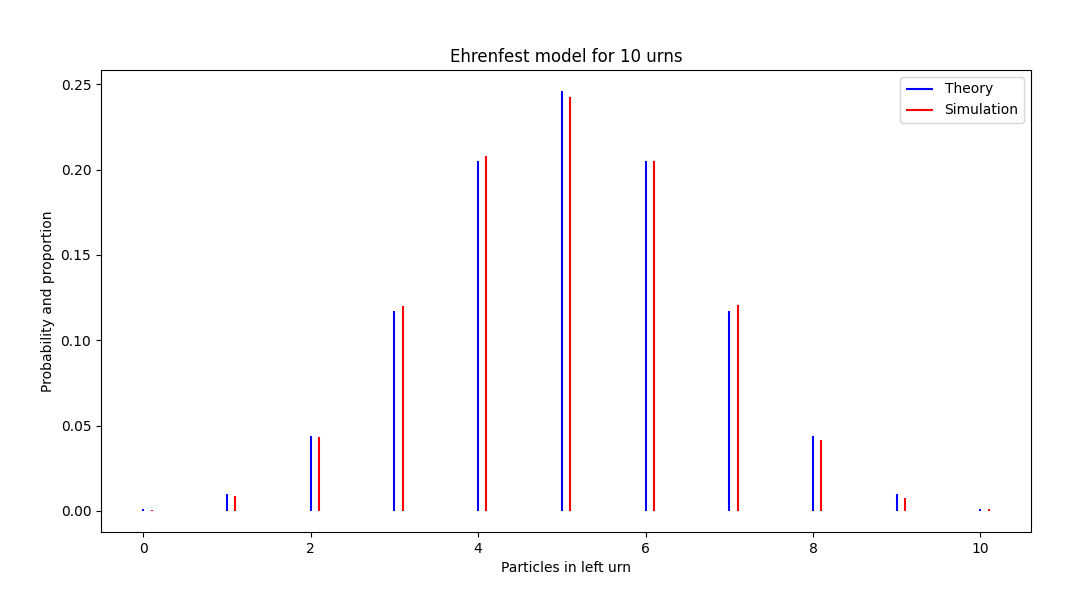
\includegraphics[width=\textwidth]{ehrenfest-01}
\caption{Stationary distribution for the Ehrenfest model}\label{f.ehrenfest1}
\end{center}
\end{figure}
